\chapter{Development}
This chapter describes in detail the main components of the simulation and how
they where implemented. How and why certain decision have been taken and alternative
solutions.

The project was developed in an iterative fashion, following with a first Prototype
after the initial literature research and evaluation of alternative simulation frameworks
(see \ref{StateOfTheArt}).

\section{Agent-based model}
As described briefly in the chapter on the State of the Art (\ref{StateOfTheArt})
a agent-based model is a multi agent simulation with a special focus on the interaction
and resulting group dynamics of its agents. The main components of a Agent-based
model are the following:

\begin{itemize}
    \item \textbf{the environment:} The environment is a strictly
    defined space in which the agents can move and interact with each other as 
    well as with other objects that are part of the environment. 
    \item \textbf{the agents:} The agents are autonomous dynamic systems with a
    set of sensors and actors that interact with each other and with the environment.
    \item \textbf{the simulation mechanics and agent logic:}  The simulation mechanics
    controls how agents interact with each other, how the environment changes
    as of actions of the agent or external factors (e.g. a simulation protocol defining
    a change in the environment). The agent logic governs the dynamic cycle between
    the agent, other agents and the environment. It defines how internal states change,
    and which behavior the agent should perform.
\end{itemize}

\subsection{Unity3d}
Unity3d[NOTE: REF] is a Computer Game Engine that has been used to develop not only
AAA (i.e. high quality [NOTE: definition]) computer games but as well is continuously
applied more and more to build simulations for commercial and academic purposes.
Unity3d is distributed under various licencees, including a Free use license, which
enables its use for Indie Game Developers as well to be applied in Academia without costs.
For our purposes Unity3d is a generic Simulation Framework that provides the tools
to create virtual 3d environments, a physics engine, a User Interface and autonomous
agents.

The simulation is implemented as a Unity3 application with a single scene that is
dynamically generated based on the simulation and classroom configuration.

All objects (Agents and Tables) in the classroom are Unity GameObjects that are
updated in defined sequence with a constant rate of 1 Hz. The agent logic is therefor
running in discrete steps, although the underlying Unity3d engine is executed
continuously (as much as this is possible on a discrete computer system).

Although not completely separated, Simulation Logic is split from game content
like Sprites (i.e. Images), Animations and other visual elements. The Simulation
Logic is implemented as C\# scripts that interface the Unity3d Framework.
During the development it was taken care to separate the Unity3d specific elements
from the rest of the simulation logic, in order to reduce dependence and make it
possible to port the Simulation Logic to other platforms.

\subsection{The environment: a classroom}
In our case the environment is classroom that contains multiple tables for
students to study individually and in small groups. In addition the environment
is modeling the noise that is accumulating in the classroom resulting from the
different actions performed by the agents.

Agents are moving about in the classroom as part of the various actions they perform.
The Unity3d Navigation Agent Infrastructure is used to control the movement of agents,
including path finding and collision control.

The noise model implemented, is accumulating the noise produced by the different actions
performed by all agents in the classroom. Different Actions produce different amount
of noise depending on the simulation configuration.

\label{agent}
\subsection{The agents: school children}

\begin{figure}[]
    \centering
    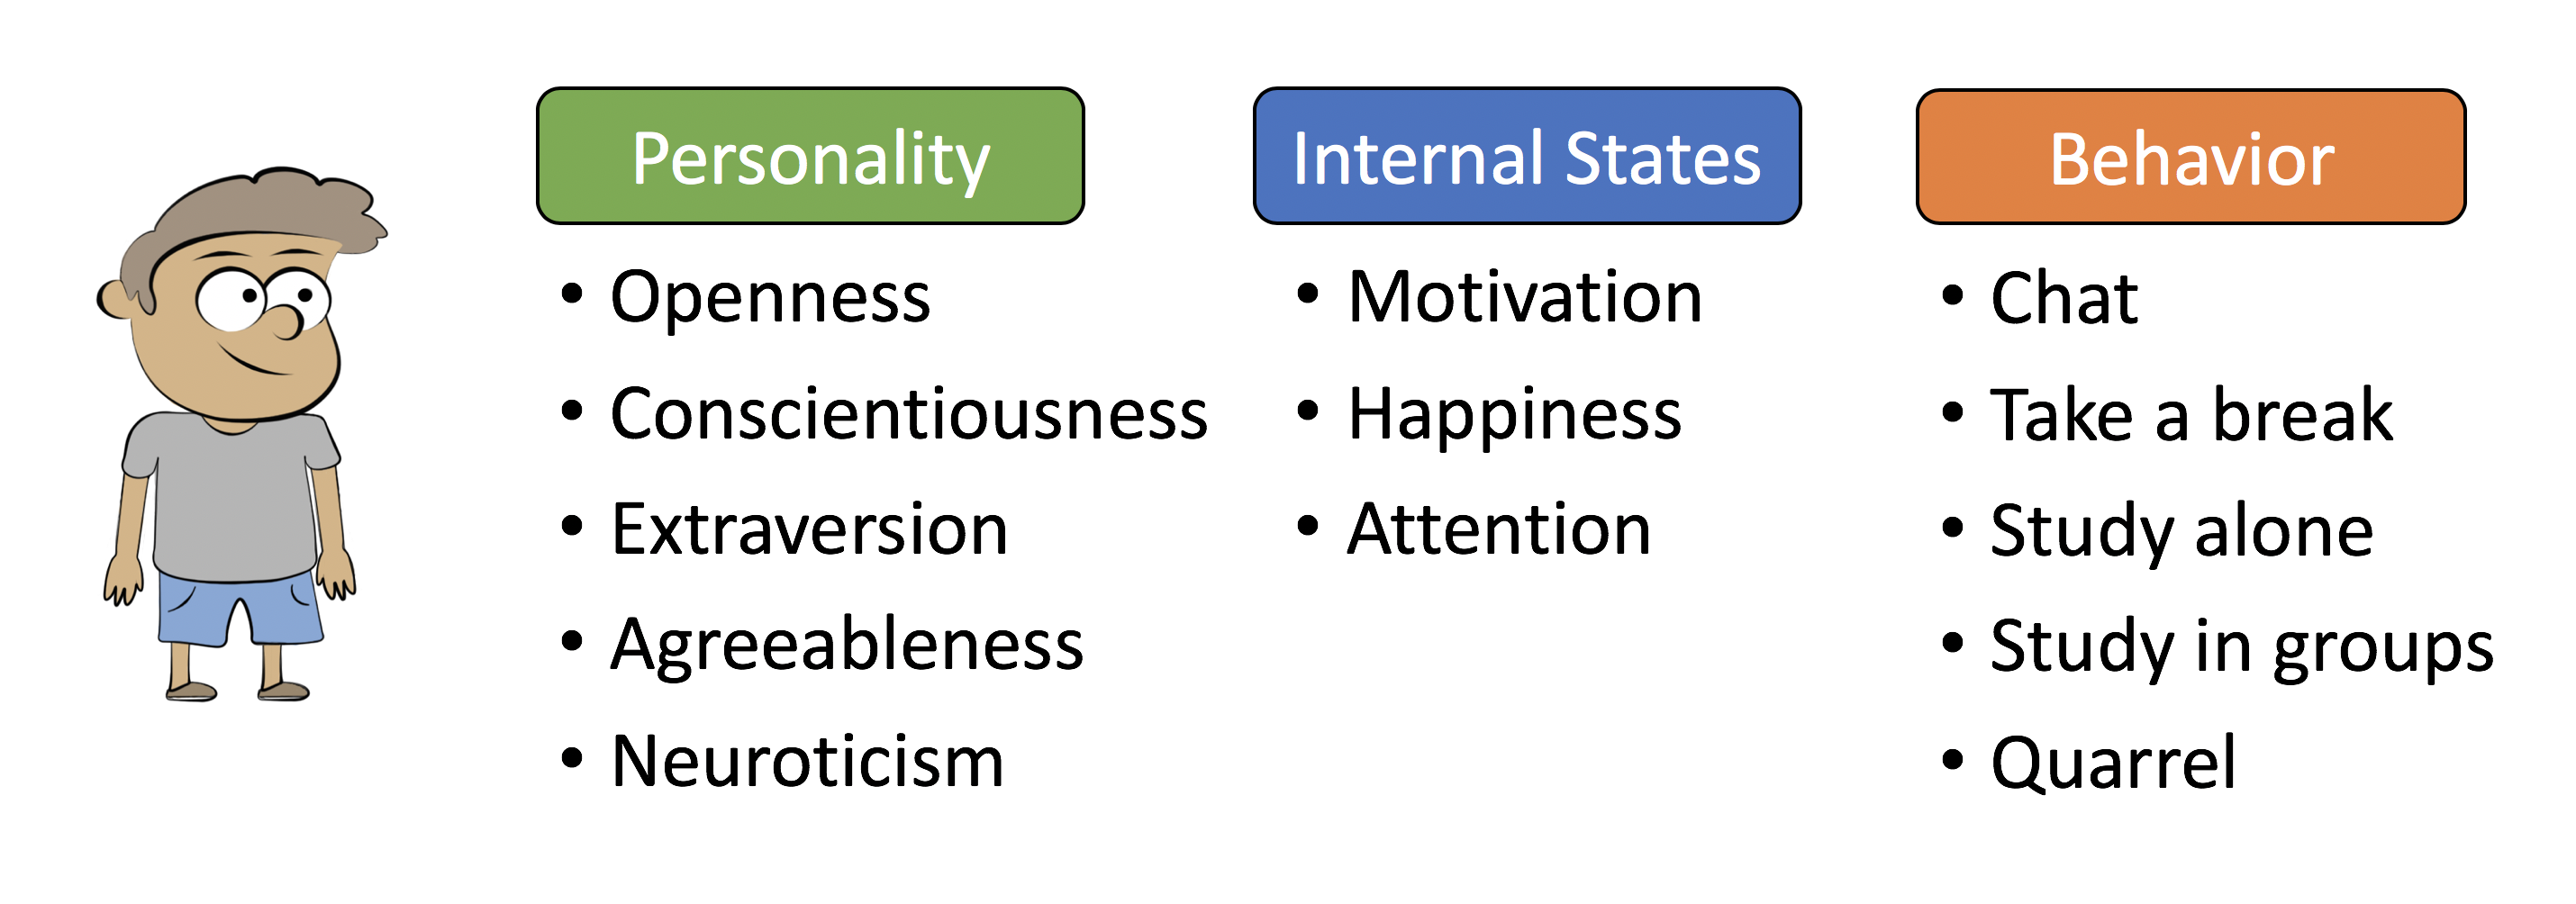
\includegraphics[width=400pt]{AgentOverview}
    \caption{Agent Overview}
    \label{AgentOverview}
\end{figure}

The agents are modeled to simulate school children of no specific age or physical
property. Instead agents are characterized by their personality traits based on 
the Big Five Personality Traits model (see \ref{BigFive}). In addition agents have
several internal states and a set of possible behaviors they can perform (see \ref{AgentOverview}).

The internal states modeled by the agent are \textbf{motivation} to study, \textbf{happiness}
and \textbf{attention} during studies.

The behaviors available to the agents fall into one of three different types, being
either educational, recreational or the conflict.

\begin{itemize}
    \item \textbf{Chat:} Agents chat with another random selected agent in the classroom.
    \item \textbf{Take a break:} Agents take a break and start a random walk through the classroom.
    \item \textbf{Quarrel:} Agents start to quarrel with another random selected agent in the classroom.
    \item \textbf{Study alone:} Agents sit down on one of the individual tables and learn by themselves.
    \item \textbf{Study in groups:} Agents take a spot on a group table and study with the other agents on the table.
\end{itemize}

All possible actions, are in one of the following states at each moment in time

\begin{itemize}
    \item \textbf{Inactive:} The action is not active at all (This is needed because of implementation details). 
    \item \textbf{Transition:} The agent is walking towards it needs to in order to perform the action.
    \item \textbf{Waiting:} The agents is waiting for either some response of another agent in order to perform the action.
    \item \textbf{Executing:} The agent is actively performing the action.
\end{itemize}

As the agents behavior depends on the internal states but as well is effecting them,
each agent itself is a \textbf{dynamics systems} that is governed by the agent logic, based
on the personality profile of the agent (see a visualization of this cycle in figure \ref{AgentDynamics}).

\begin{figure}[]
    \centering
    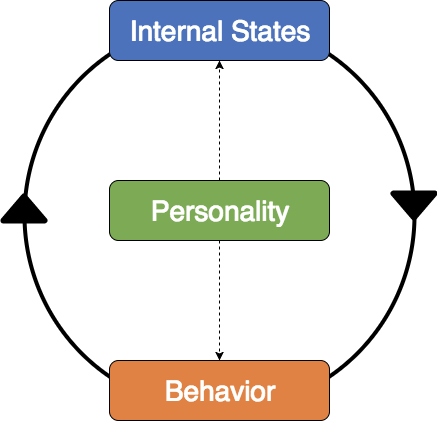
\includegraphics[width=200pt]{AgentDynamics} 
    \caption{Agent Dynamics}
    \label{AgentDynamics}
\end{figure}

\subsubsection{Dynamic Systems}
As mentioned in the introduction, agent-based models are focus on the interaction
\textit{between} components of the simulation. The complete system is therefore
the result of the interaction of multiple dynamic systems (i.e. agents and environment)
(see figure \ref{GroupDynamics}). 

\bb

This \textbf{multi level dynamic system} can express very sophisticated behavior and dynamics,\
making it one of the main reasons agent-based models are such a powerfully tool to study
real world phenomena. One of the most curious aspects of complex dynamic systems
are \textbf{emergent phenomena}\cite{Corning2002} which describes aspects of the
complete system (i.e. classroom), absent in the individual (i.e. children) components.

\bb

One examples of emerging properties is the \textit{wetness} of Water that only appears in a
ensemble of many water molecules, not present in a single individual molecule. 
Another famous example is \textbf{Cowans Game of Life}\cite{Adamatzky2010}
that shows the almost infinite complexity generated by a cellular automata simulating
black or white cells on a infinite grid. Constructs generated by the simulation
have emerging properties like \textit{self replication}, \textit{finite} and
\textit{infinite cycles} and many more. None of those behaviors are obviously deducible
from the initial basic interaction rules. Instead those properties emerge in the
interaction between the rules 'agents' (using agent in an amplified sense here)
following basic rules.

\begin{figure}[]
    \centering
    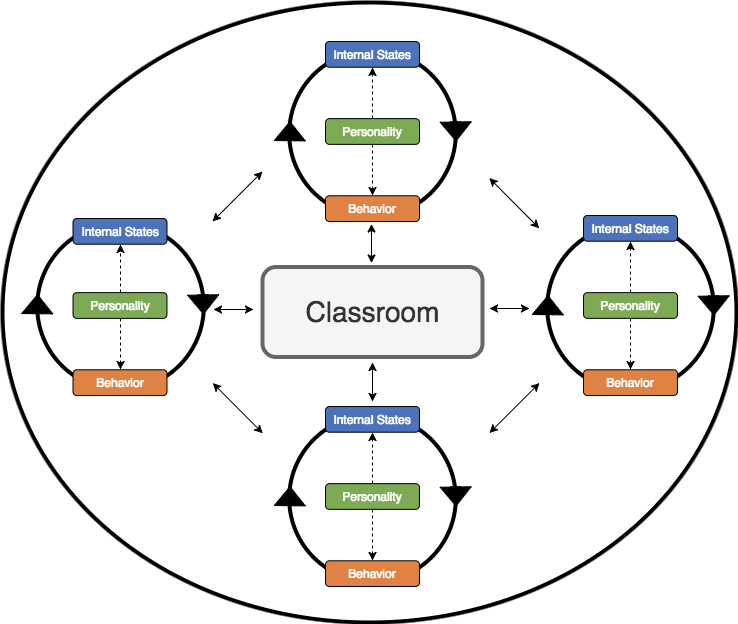
\includegraphics[width=200pt]{GroupDynamics} 
    \caption{Group Dynamics}
    \label{GroupDynamics}
\end{figure}

\subsubsection{Agent homogeneity}
One axis along which to classify agent-based models is agent homogeneity\cite{Pudane2017}.
In homogeneous agent models all agents share the same characteristic's and agent logic.
Heterogeneous agent models on the other side can differ in the agents logic, its behavior
or based on some parameters in its configuration.

In our case the simulation contains heterogeneous agents that differ, based on parameters
in their Personality Traits. 

\label{BigFive}
\section{Agent Personality Traits}
As described earlier each agent is a dynamic system that in which the internal states
interact with the agents behavior. Those interactions are governed by the agent logic
witch is based on the \textbf{Personality Traits} of the agent.

It is not novel to use personality traits in ABM, but previous works\cite{Gautam2009}
modeled very abstract personality traits that have no relation to the real world.

We therefore where careful, to chose an established and widely used personality traits model.
The \textbf{OCEAN} personality trait model\cite{Tupes1961}, common known as the \textbf{Big-Five}, has been developed
in the 1960s and has since been used in applied and theoretical psychology.
It is based on factor analysis of empirical studies (mostly self description of patients about their
behavior and self image).

Its name is derived from the five orthogonal dimensions which are used to describe
the personality of an individual, where the extremes of each dimension are associated
with typical behaviors or thought patterns (see figure \ref{OCEAN-Model} for a graphical
representation).

A short description of the different dimension has been taken from\cite{Ehrler1999}
(see table \ref{OCEAN-Model-table} ).

Although the personality traits of a person could change over time, there is strong
evidence (\cite{Soldz1999}, \cite{Cobb-Clark2012}) that the personality traits of
the big five model stay more or less constant over a long period of time or even
the complete life of an individual.

\begin{figure}[h]
    \centering
    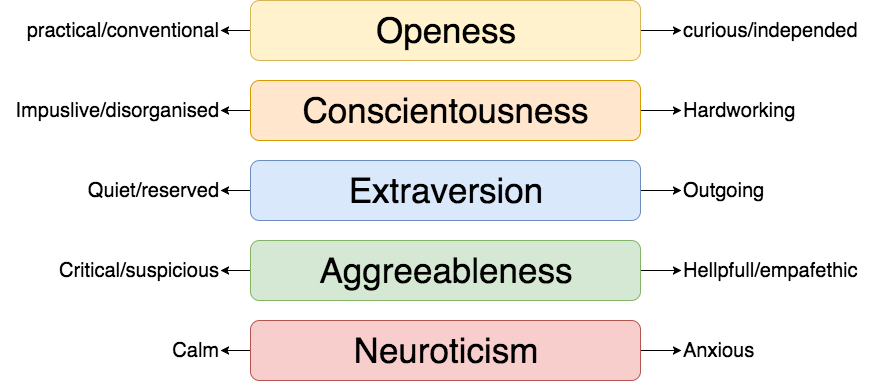
\includegraphics[width=400pt]{OCEAN-model} 
    \caption{OCEAN Model}
    \label{OCEAN-Model}
\end{figure}

\begin{table}[]
\begin{tabularx}{1.2\textwidth}{|>{\hsize=.2\hsize}X|X|}
    \hline
    \multicolumn{1}{|c|}{\textbf{Personality Trait}} & \multicolumn{1}{c|}{\textbf{Description}} \\
    \hline
    
    Openess & The general tendency to be curious about both inner and outer worlds.
    O includes the elements of an active imagination, aesthetic sensitivity,
    attentiveness to inner feelings, preference for variety, intellectual
    curiosity, and independence of judgment. A high O also includes individuals
    who are unconventional, willing to question authority, and ready to entertain
    new ethical and social ideas. \\
    \hline
    
    Conscientiousness & The general tendency to be able to resist impulses and
    temptations. The conscientious individual is purposeful, strong-willed, and
    determined.
    On the positive side, high C is associated with academic and occupational
    achievement; on the negative side, it may lead to annoying
    fastidiousness, compulsive neatness, or workaholic behavior, Low C’s are not
    necessarily lacking in moral principles, but they are less exacting
    in applying them. \\
    \hline
    
    Extraversion & The general tendency to be outgoing. In addition, high E’s
    prefer large groups and gatherings and are assertive, active, and talkative.
    They like stimulation and tend to be cheerful in disposition. They are upbeat,
    energetic, and optimistic. \\ 
    \hline
    
    Agreeableness & The general tendency to be altruistic. The high A is
    sympathetic to others and eager to help them, and believes that others will
    be equally
    helpful in return. By contrast, the low A is antagonistic and egocentric,
    skeptical of others’ intentions, and competitive rather than cooperative. \\
    \hline
    
    Neuroticism & The general tendency to experience negative affects such as fear,
    sadness, embarrassment, anger, guilt, and disgust is the core of the N domain. 
    However, N includes more than susceptibility to psychological distress. Perhaps
    because disruptive emotions interfere with adaptation, those
    who score high in N are also prone to have irrational ideas, to be less able
    to control their impulses, and to cope more poorly then others with stress. \\
    \hline
  \end{tabularx}
  \label{OCEAN-Model-table}
  \caption{Ocean model factors taken from \cite{Ehrler1999}}
\end{table}

\subsubsection{Big-five in the classroom}
Various empirical studies have been performed in the past in order to investigate
the association between Personality Traits, behavior and academic outcome in schools
(\cite{Ehrler1999}, \cite{Nigg2002}, \cite{Asendorpf2003}).
We used those empirical found associations to define and tune agent logic as well
as simulation parameters in order to reproduce agent behavior that is in agreement
with those results.

Although it is well studies how the Big-Five behave on an individual level, we
found very few studies that focused on group dynamics influenced by the
Big-Five. One work that we did find\cite{Selfhout2010} studied how the Big-Five
influence the forming of new friendships in adolescence, but limited the study
to pair wise interactions.

We know of no other study besides ours that focuses on the modulation of group
dynamics based on personality trait variations.

\section{Agent Logic}
The agent logic is identical for all agents, but the internal states and
states related to the agent behavior is maintained separately per agent.

The Logic is implemented as a infinite loop, repeating the following steps

\begin{enumerate}
    \item \textbf{Calculating action score}
    \item \textbf{Action selection}
    \item \textbf{Action execution}
    \item \textbf{Handling interactions}
    \item \textbf{Updating internal states}
\end{enumerate}

\subsubsection{Calculating action score}
The agent can execute one of five actions (see the section about \ref{agent}).
Independent of each other a score is calculated for each action. Tjat score is than
used to select which action to perform. Section \ref{action-scores} covers the
action score calculation in detail, for now it suffice to say that the score of
an action depends on the the internal states of the agent and its psychological
profile.

\bb

Besides the action score, the agent is calculating an \textbf{action score bias}
that is added to the score of the current action and subtracted from the score
of the previous action. This mechanism is used to keep the agent from switching
between actions too quickly, and in case of the added bias models the tendency to
continue with an ongoing task (similar to sustaining attention). The previous
action score is reduced in order to keep the agent from looping between possible
actions, and cause a more diverse action selection.

\bb

The action bias depends on the conscientiousness of the agent and is following an
exponential decay curve, where time is the number of ticks the agent is performing
the current action. The number of ticks is only counted as the action is executed,
not in its other states, making sure that Transitions or Waiting do not effect the
action score bias.

\begin{equation}
    \label{eq1}
    scorebias(a_i) = A * e^{-(1.0 - c) * t}
\end{equation}
with
\begin{itemize}
    \item $a_i$ is the action i
    \item where A is a simulation parameter defining the maximum bias
    \item where c is the agents conscientiousness
    \item where t is the number of ticks the current task is executed
\end{itemize}

\subsubsection{Action selection}
Once the actions are scored a single action is selected probabilistically. The
probability for a action to be selected is defined by the square of the normalized
action scores (see equation \ref{eq2}). Taking the squared action score makes sure
that the highest rated score has a clear advantage over the other actions, but still
gives other actions a chance to be selected.

\begin{equation}
    \label{eq2}
    p(a_i) = \frac{s_i^2}{\sum s_i^2} \\
\end{equation}

with
\begin{itemize}
    \item $p(a_i)$ is the probability of action i to be selected
    \item where $s_i$ is the score for action i
\end{itemize}


\subsubsection{Action execution}
For the selected action it is tested if it can be performed, and if this is possible
than the action is executed. Otherwise, the agent is taking a break, which works
as the default action. In addition if it is not possible to perform an action, the
agent keeps track of what its desired action is, and what the action that is actually
executing. 

\subsubsection{Handling Interaction}
Some of the agent behaviors like chat and quarrel depend on direct interactions
between actions. Meaning that if agent A want to chat with agent B (that is
randomly selected from the available agents), than Agent A depends on B
\textit{accepting} its invitation to chat. This mechanism is implemented
by agent A is sending a request for chatting to agent B, and agent B decides to
either accept or reject the invitation. 

In case the request is accepted the agents perform the action (i.e. chat or quarrel),
and if not, the sending agent A will retry either sending another request to the
same agent B, or to another agent randomly selected.

\bb

The receiving agent B will interrupt any ongoing action and join the interaction.
The decision if the agent B accepts the interaction os not depends on its personality
traits. In case of chat the relevant personality trait is conscientiousness and
in case of quarrel agreeableness. For each interaction a random number between
0.0 and 1.0 is generated. The that number is bigger than the corresponding personality
trait of B, the interaction is accepted.

This mechanism makes sure to reflect the empirical findings that agents with a high
level of conscientiousness are less likely to be distracted from the active task,
and that high level of agreeableness is associated with less involvement in conflicts.

\subsubsection{Updating internal states}
The last step of the agent logic loop is to update the internal states of the agent.

From the free internal states motivation, attention and happiness, only two (attention
and happiness) are updated at this step.

\begin{enumerate}
    \item \textbf{Happiness:} is increased if the current action is not quarrel,
    and the executed action is identical to the desired action. In case the agent
    is executing a not desired action happiness is decreased by a factor that is
    scaled by the agents neuroticism. The happiness increment is a simulation parameter.
    \item \textbf{Attention:} In case the agent is studying (either alone or in a group),
    its attention is calculated by calculating the sum of its motivation plus conscientiousness
    minus the noise in the classroom.
\end{enumerate}

As for motivation, this internal state is altered by the action performed.

\label{action-scores}
\subsection{Actions Scores}
